\documentclass[12pt]{article}

\usepackage[spanish]{babel}
\usepackage[utf8]{inputenc}
\usepackage{graphicx}
\usepackage{geometry}
\usepackage{xcolor}
\usepackage{fancyhdr}
\usepackage{lastpage}
\usepackage{pdfpages}
\usepackage{listings}

\geometry{top=25mm,left=15mm,right=15mm,a4paper}

\pagestyle{fancy}
\fancyhf{}
\lhead{Sistemas Operativos}
\cfoot{Página \thepage\ de \pageref{LastPage}}

\graphicspath{./}

\begin{document}
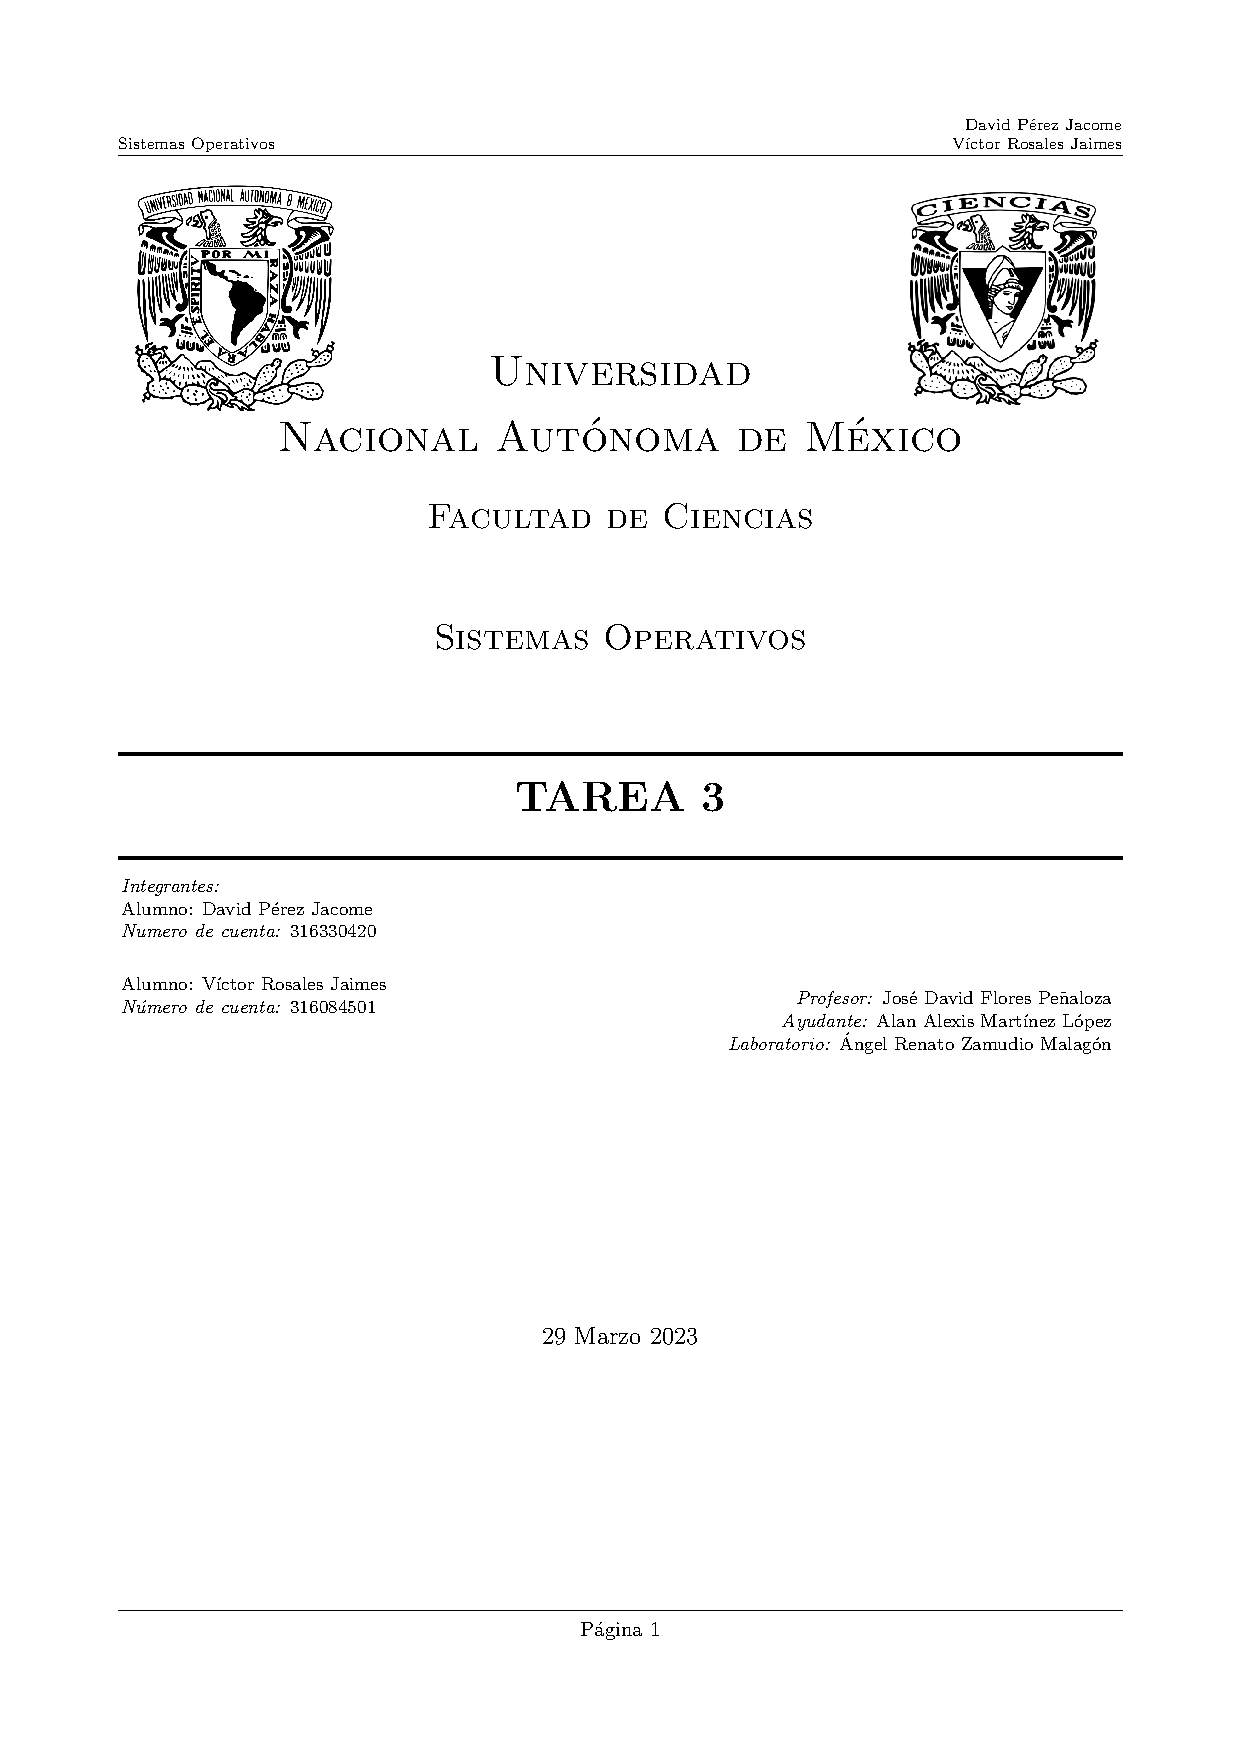
\includepdf{Portada.pdf}
{\color{blue} \section*{Tarea 4.}}

{\color{blue} \subsection*{Instrucciones.}}
\vspace{0.5em} 

Lee con atención las preguntas y contesta lo correspondiente. La tarea se entregará por vía classroom
en un archivo pdf que debe tener el nombre completo y número de tarea, ya sea en una portada o en el encabezado.
\textbf{La tarea se entregará en equipos a lo más de dos personas.}\\

{\color{blue} \subsection*{Ejercicios}}
\vspace{0.5em}

\begin{enumerate}
    \item Describe a detalle la inversión de prioridad de procesos.
    \vspace{2mm}

    \textbf{Cuando ocurre la llamada inversión de prioridades es cuando tenemos el caso de un proceso de menor prioridad retrasa a uno de mayor prioridad y lo deja esperando.
    $Prior(T_3) < Prior(T_2) < Prior(T_1) $ y $T_1$ espera a que termine $T_3$ y $T_2$}

    \item Dada la inversión de prioridad de procesos. ¿Qué inconvenientes tiene? ¿Cómo se podría solucionar?
    \vspace{2mm}
    
    \textbf{El principal inconveniente que tiene es que se deja un proceso de alta prioridad esperando usar el recurso compartido, una posible solución a este problema es la llamada Donación de prioridades que
    consiste en cuando un proceso de alta prioridad solicita un recurso que está siendo utilizado por un proceso de baja prioridad, la prioridad del proceso de baja prioridad se eleva temporalmente (le prestan) a la del proceso de alta prioridad.}
    
    \item ¿Qué es la memoria caché? ¿Para qué sirve?.
    \vspace{2mm}

    \textbf{La memoria caché es uno de los recursos con los que cuenta una CPU para almacenar temporalmente datos recientemente procesados un una memoria auxiliar. Una memoria estática de acceso aleatorio, muy rapida y localizada cerca de la CPU.
    Y su principal función es almacenar datos o Instrucciones que la CPU necesitará en el futuro inmediato, se gana velocidad en la ejecución de procesos evitando que la CPU espere. Mejora el rendimiento y velocidad de la CPU.}

    \item ¿Qué es el \textbf{base register} y el \textbf{limit register} respecto al espacio de memoria de cada proceso?
    \vspace{2mm}
    \textbf{\begin{enumerate}
        \item Registro base o base register: Tiene la dirección de memoria física de inicio del proceso 
        \item Registro limite o limit register: Especifica el tamaño maximo del segmento.
    \end{enumerate}}

    \item Describe con detalle qué es swapping y por qué es necesario. 
    \vspace{2mm}

    \textbf{En las direcciones tenemos bits administrativos, como uno que indica que si tenemos una pagina presente o no en memoria.
    Si no la encuantra, manda una interrupción para que el kernel tenga control y obtenga la pagina del disco duro, si hay espacio en memoria se coloca si no repite el proceso.
    Lo que se hace principalmente es que en swapping movemos momentaneamente parte del contenido de la memoria principal a la memoria secundaria.}

    \item Explica qué es segmentación, describe pros y contras.
    \vspace{2mm}

    \textbf{RESPUESTA}

    \item ¿Qué es la tabla de segmentos?  
    \vspace{2mm}

    \textbf{RESPUESTA}

    \item Explica qué es la MMU
    \vspace{2mm}

    \textbf{Es la Memory Managent Unit, es un componente de hardware que se utiliza para administrar el acceso a la memoria física por parte de los procesos del sistema operativo. 
    Su función principal es traducir las direcciones virtuales utilizadas por los procesos en direcciones físicas que puedan ser utilizadas por el hardware de la computadora.}
    
    \item Explica qué es paginación, describe pros y contras.
    \vspace{2mm}

    \textbf{La paginación en pocas palabras es un mapeo fleible inyectivo, espacio virtual se divide en paginas y el fisico en direcciones y mapea de virtual a fisico.
    Se trata de un modelo de organización de memoria física en el que se divide toda la memoria en porciones del mismo tamaño. Esas porciones reciben el nombre de marcos o páginas físicas. Si dividimos la memoria en páginas, podremos gestionarla mejor.
    \begin{enumerate}
        \item Pros: Es posible comenzar a ejecutar un programa, cargando solo una parte del mismo en memoria, y el resto se cargara bajo la solicitud.
        Facil control de paginas por tener mismo tamaño.
        \item Contras: El costo de hardware y software se incrementa, por la nueva información que debe manejarse y el mecanismo de traducción de direcciones necesario. Se consumen muchos más recursos de memoria, tiempo en el CPU para su implantación.
    \end{enumerate}}

    \item ¿Qué es compartición?
    \vspace{2mm}
    
    \textbf{Los procesos deben de compartir memoria (relacion productor.consumidor), instancias de un programa pueden compartir una sola copia del programa.}

    \item ¿De qué manera determinas a que página pertenece una dirección virtual en paginación?
    \vspace{0mm}
    \textbf{Mediante una tabla de paginación que contiene información sobre la página, incluyendo la dirección física de la página correspondiente y otros bits de control para indicar si la página está presente en memoria física, si se ha modificado, etc.}

    \item ¿Qué es un frame y qué es un page? ¿Cúal es su relación?
    \vspace{2mm}
    
    \textbf{\begin{enumerate}
        \item Frame: Un frame es un bloque de memoria física de tamaño fijo que se utiliza para almacenar una página de memoria virtual en la memoria física. Cada frame tiene una dirección física única.
        \item Page: Una page es una unidad de memoria virtual de tamaño fijo que se utiliza para dividir la memoria virtual de un proceso en bloques más pequeños que se pueden almacenar en la memoria física. Cada page tiene una dirección virtual única.
    \end{enumerate}}

    \item Describe la paginación de varios niveles y que beneficios tiene en comparación a la paginación normal.
    \vspace{2mm}
    
    \textbf{La paginación de varios niveles es una técnica utilizada en la administración de la memoria virtual para manejar grandes espacios de direcciones virtuales. Esta técnica utiliza varias tablas de páginas anidadas para permitir la asignación dinámica de memoria de forma más eficiente y flexible que la paginación de un solo nivel.
    Entre los beneficios tenemos que en lugar de tener una gran tabla de páginas para cada proceso, la paginación de varios niveles divide la tabla de páginas en varias tablas de páginas más pequeñas. Esto reduce la sobrecarga de la tabla de páginas y hace que la administración de la memoria virtual sea más eficiente.
    Aunque al tener multiples niveles hay un aumento en el acceso a memoria.}

    \item Explica la técnica que se usa para mitigar los efectos negativos de usar múltiples niveles en la técnica de paginación.
    \vspace{2mm}
    
    \textbf{La solución es usar TLB (Tabla asociativa o Translation Lookaside Buffer) La cual es una memoria caché de hardware que almacena una copia de las entradas de la tabla de páginas utilizadas más recientemente para la traducción de direcciones virtuales.
    Y asi tener un rapido acceso a estas localidades, se encuantra dentro de la MMU (registros internos).}

    \item ¿Qué es el TLB (Translation Lookside Buffer)?
    \vspace{2mm}
    
    \textbf{Es la Translation Lookaside Buffer, es una memoria caché administrada por la unidad de gestión de memoria (MMU), que contiene partes de la tabla de paginación, la cual relaciona las direcciones lógicas con las físicas. Posee un número fijo de entradas y se utiliza para obtener la traducción rápida de direcciones.
    Cada entrada es de 2 campos: $<No.pagVirtual, No.pagFisica>$}

    \item Dada la siguiente cadena de referencia: $4,7,5,3,2,3,5,3,7,6,0,1,4,0,7,1,6.$ Realiza el algoritmo de FIFO Page Replacement con 4 Frames
    \vspace{2mm}
    
    \textbf{RESPUESTA}

    \item Dada la siguiente cadena de referencia: $4,7,5,3,2,3,5,3,7,6,0,1,4,0,7,1,6.$ Realiza el algoritmo de Optimal Page Replacement con 4 Frames.
    \vspace{2mm}
    
    \textbf{RESPUESTA}

\end{enumerate}

\end{document}